% !TeX root = ../main.tex
\chapter{Unidad 9: Factores que afectan la propagación del sonido}
\label{chap:unidad-9}

\section{Propósito y resultados de aprendizaje}
\label{sec:u9-proposito}

Entre una fuente y un receptor no existe solamente una distancia. El sonido
puede propagarse en un medio cuyas propiedades cambian con la altura, encontrar
superficies y obstáculos, atravesar cerramientos y alcanzar un recinto por
rutas diferentes. Por eso, un nivel emitido por una fuente no determina por sí
solo el nivel que se recibirá en otro punto.

Esta unidad aplica los modelos ideales presentados en capítulos anteriores a
la propagación ambiental, los recintos y las cabinas audiométricas. La
descripción se mantiene en un nivel introductorio: permite reconocer
mecanismos, realizar estimaciones y justificar mediciones, pero no sustituye
el cálculo profesional de una instalación ni un procedimiento normativo.

Al finalizar la unidad se espera que podamos:

\begin{itemize}
    \item aplicar el cambio de nivel con la distancia sin volver a derivar la
    ley del cuadrado inverso y declarar cuándo el modelo deja de ser adecuado;
    \item interpretar el factor de directividad \(Q\) y el índice de
    directividad \(DI\) sin sumar dos veces el efecto de la fuente;
    \item distinguir un estado atmosférico uniforme de un gradiente de
    temperatura o de viento y explicar cualitativamente la refracción
    resultante;
    \item separar pérdida por divergencia geométrica, absorción atmosférica,
    reflexión, absorción material, transmisión y difracción;
    \item diferenciar acondicionamiento acústico, aislamiento acústico e
    insonorización;
    \item interpretar la ley de masas como un modelo aproximado para una pared
    simple, con sus supuestos y limitaciones;
    \item describir una cabina audiométrica como un sistema de cerramientos,
    uniones, accesos, ventilación y control del ruido interior;
    \item explicar por qué el ruido ambiente máximo permitido para una
    audiometría no puede reducirse a un único valor en \(\text{dB(A)}\).
\end{itemize}

\section{Conocimientos previos}
\label{sec:u9-previos}

La unidad utiliza cuatro grupos de conocimientos ya desarrollados:

\begin{itemize}
    \item la temperatura, la densidad y la velocidad de propagación en gases,
    tratadas en la Sección~\ref{sec:u2-temperatura-velocidad};
    \item la longitud de onda y la relación \(c=\lambda f\), presentadas en el
    Unidad~\ref{chap:unidad-3};
    \item los niveles acústicos, el campo libre, la ley del cuadrado inverso y
    la directividad, desarrollados en las
    Secciones~\ref{sec:u4-tipos-campo}--\ref{sec:u4-directividad};
    \item el análisis por bandas y la medición con sonómetro, introducidos en
    la Unidad~\ref{chap:unidad-5}.
\end{itemize}

Conviene mantener además una distinción perceptual. Una disminución del nivel
de presión sonora es un cambio físico medible. La disminución de la sonoridad
percibida depende también de la frecuencia, la duración, el espectro, el
oyente y el contexto, como se estudió en la Unidad~\ref{chap:unidad-7}.

\section{Situación introductoria: una fuente, varios trayectos}
\label{sec:u9-situacion}

Una clínica se encuentra próxima a una calle transitada. En un consultorio se
registra un nivel mayor cuando una ventana queda abierta; en otro, el ruido se
percibe principalmente a través de la puerta y del sistema de ventilación. En
una cabina, las superficies interiores reducen las reflexiones, pero eso no
garantiza que el ruido exterior quede suficientemente atenuado.

Antes de proponer una solución conviene separar tres partes:

\begin{enumerate}
    \item la \textbf{fuente}, caracterizada por su emisión, su espectro y su
    directividad;
    \item el \textbf{trayecto}, donde actúan distancia, atmósfera, suelo,
    obstáculos, superficies, cerramientos y rutas laterales;
    \item el \textbf{receptor}, que puede ser un micrófono, un sonómetro, una
    persona o el punto de referencia de una medición audiométrica.
\end{enumerate}

La pregunta organizadora de la unidad será: ¿qué parte del cambio observado
pertenece a la fuente, cuál al trayecto y cuál a la condición de medición?

\section{Distancia, directividad y nivel recibido}
\label{sec:u9-distancia-directividad}

\subsection{Recordatorio de la divergencia geométrica}
\label{sec:u9-divergencia}

La Sección~\ref{sec:u4-cuadrado-inverso} derivó la ley del cuadrado inverso
para una fuente puntual ideal en un medio homogéneo, sin pérdidas y en campo
libre. Aquí solo se recordará su aplicación al nivel de presión sonora.

Sean \(L_{p1}\) y \(L_{p2}\) los niveles de presión sonora, expresados en
\(\text{dB SPL}\), medidos en una misma dirección a las distancias \(r_1\) y
\(r_2\), respectivamente. Ambas distancias se expresan en metros
\((\text{m})\). Bajo las condiciones indicadas,

\begin{equation}
    L_{p2}
      =L_{p1}-20\log_{10}\!\left(\frac{r_2}{r_1}\right).
    \label{eq:u9-distancia}
\end{equation}

El cociente \(r_2/r_1\) es adimensional. Si la distancia se duplica, el nivel
disminuye aproximadamente \(6{,}02\,\text{dB}\). Esta disminución representa
la redistribución geométrica de la energía sobre un área mayor; no representa
absorción atmosférica.

\subsubsection*{Ejemplo resuelto: duplicación de la distancia}

En un punto de un campo aproximadamente libre se miden
\(L_{p1}=90\,\text{dB SPL}\) a \(r_1=0{,}50\,\text{m}\). Se desea estimar el
nivel a \(r_2=1{,}00\,\text{m}\), en la misma dirección y sin cambiar la
fuente:

\[
    L_{p2}
      =90-20\log_{10}\!\left(\frac{1{,}00}{0{,}50}\right)
      \approx90-6{,}02
      \approx83{,}98\,\text{dB SPL}.
\]

Redondeado al decibel, el resultado es \(84\,\text{dB SPL}\). El cálculo
estima un nivel en otro punto; no constituye por sí mismo una calibración
audiométrica. En un recinto real también pueden intervenir reflexiones, campo
próximo, directividad y pérdidas adicionales.

\subsection{Directividad: qué se compara}
\label{sec:u9-directividad}

La Sección~\ref{sec:u4-directividad} definió el factor de directividad
\(Q(\theta,\phi)\), adimensional, y el índice de directividad
\(DI(\theta,\phi)\), expresado en decibeles. Los ángulos \(\theta\) y \(\phi\)
identifican una dirección. La relación entre ambos descriptores es

\begin{equation}
    DI(\theta,\phi)
      =10\log_{10}\!\left[Q(\theta,\phi)\right].
    \label{eq:u9-indice-directividad}
\end{equation}

La comparación se realiza a igual potencia acústica total y a igual distancia.
En campo lejano, con el mismo medio y condiciones compatibles, un \(DI\)
positivo en una dirección no implica creación de energía: indica que la fuente
redistribuye una mayor parte de su potencia hacia esa dirección.

La directividad de una fuente real depende de la frecuencia, de su
geometría, de su montaje y de las superficies próximas. Un único valor de
\(Q\) no describe por completo una fuente de banda ancha~\cite{xiangBlauert2021,iso9613_1_1993}.

Las Figuras~\ref{fig:u4-propagacion-esferica} y
\ref{fig:u4-directividad-q} permiten comparar la divergencia geométrica con
la redistribución direccional de la potencia. Se las retoma aquí para aplicar
ambos conceptos sin duplicar su desarrollo.

\subsubsection*{Ejemplo resuelto: comparación a igual potencia}

Se comparan dos fuentes a la misma distancia y con la misma potencia acústica
total. En la dirección de interés, una es omnidireccional
\((Q_\mathrm{o}=1)\) y la otra posee \(Q_\mathrm{d}=4\). Para la fuente
direccional,

\[
    DI_\mathrm{d}
      =10\log_{10}(4)
      \approx6{,}02\,\text{dB}.
\]

Dentro del modelo, el nivel en esa dirección es aproximadamente
\(6{,}02\,\text{dB}\) mayor que el de la fuente omnidireccional de igual
potencia. Si en cambio se informa un nivel ya medido en esa dirección, no se
debe volver a sumar \(DI_\mathrm{d}\).

\subsection{Nivel de emisión y nivel recibido}
\label{sec:u9-emision-recepcion}

Sea \(W\) la potencia acústica emitida, expresada en watts \((\text{W})\), y
sea \(W_0\) una potencia de referencia expresada en la misma unidad. El nivel
de potencia acústica \(L_W=10\log_{10}(W/W_0)\), expresado en decibeles,
describe la emisión total de una fuente. El nivel de presión sonora \(L_p\),
expresado en \(\text{dB SPL}\) cuando se utiliza la referencia de presión del
aire, describe el campo en un punto. No son la misma magnitud.

En una situación real, el nivel recibido depende de la emisión de la
fuente, su directividad, la divergencia geométrica, la absorción del medio, las
interacciones con el suelo y las superficies, los obstáculos, las rutas de
transmisión y la posición del receptor~\cite{xiangBlauert2021,iso9613_1_1993}. La ecuación~\eqref{eq:u9-distancia}
solo representa uno de esos términos.

\section{Condiciones atmosféricas}
\label{sec:u9-atmosfera}

\subsection{Temperatura uniforme y gradientes térmicos}
\label{sec:u9-temperatura}

La temperatura uniforme modifica la velocidad de propagación, mientras que un
gradiente de temperatura puede modificar además la dirección del trayecto.
Estas dos situaciones no deben confundirse.

Para aire seco y temperaturas próximas a las ambientales puede usarse
como aproximación didáctica~\cite{xiangBlauert2021,iso9613_1_1993}

\begin{equation}
    c\approx
    331\,\text{m}/\text{s}
    +\left(0{,}6\,
    \frac{\text{m}/\text{s}}{^{\circ}\text{C}}\right)\vartheta,
    \label{eq:u9-velocidad-temperatura}
\end{equation}

donde \(c\) es la velocidad de propagación, expresada en metros por segundo
\((\text{m}/\text{s})\), y \(\vartheta\) es la temperatura ambiental,
expresada en grados Celsius \((^{\circ}\text{C})\). La ecuación recuerda el
modelo ya presentado en la Unidad~\ref{chap:unidad-2} y no debe extrapolarse
fuera del intervalo
en el que se valide.

Si la temperatura es uniforme, una frecuencia \(f\), expresada en hertz
\((\text{Hz})\), conserva el valor fijado por la fuente. El cambio de \(c\)
modifica la longitud de onda \(\lambda=c/f\), expresada en metros
\((\text{m})\), pero no transforma automáticamente la frecuencia en otra
altura tonal.

Cuando \(c\) cambia con la altura, un modelo de rayos acústicos predice
curvatura hacia las regiones de menor velocidad de propagación. Un suelo
calentado durante el día puede producir curvatura ascendente y una región de
sombra cerca del suelo; una inversión térmica nocturna puede producir
curvatura descendente y favorecer trayectos hacia receptores distantes~\cite{xiangBlauert2021,iso9613_1_1993}.
Estas descripciones son cualitativas: el resultado también depende de la
geometría, el suelo y el perfil atmosférico real.

La Figura~\ref{fig:u9-gradientes-termicos} compara los dos sentidos de
curvatura. Las trayectorias representan un modelo de rayos y no el
desplazamiento de porciones identificables de aire.

\begin{figure}[htbp]
    \centering
    % Propósito: comparar la refracción por dos perfiles térmicos opuestos.
% Origen: c(z) depende de la temperatura; los rayos se curvan hacia la
% región de menor velocidad. Esquema cualitativo, sin datos experimentales.
% Accesibilidad: dos paneles muestran suelo cálido con curvatura ascendente
% y una inversión térmica con curvatura descendente.
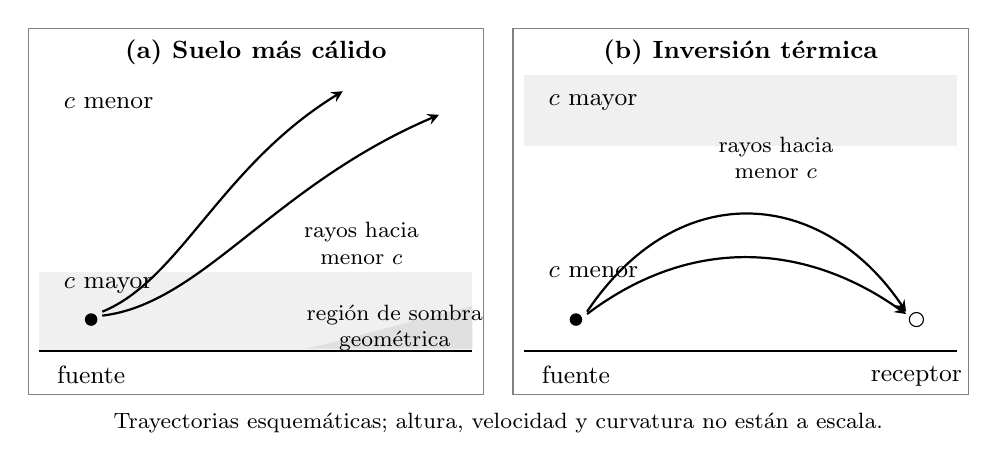
\begin{tikzpicture}[
    x=0.94cm,
    y=1cm,
    >=stealth,
    font=\small,
    rayo/.style={thick,->},
    guia/.style={gray,dashed},
    banda/.style={fill=black!6,draw=none}
]
    % Panel diurno
    \draw[gray] (0,0) rectangle (6.15,4.65);
    \node[font=\small\bfseries] at (3.075,4.35) {(a) Suelo más cálido};
    \path[banda] (0.15,0.55) rectangle (6.0,1.55);
    \draw[thick] (0.15,0.55) -- (6.0,0.55);
    \node[anchor=west] at (0.35,1.38) {\(c\) mayor};
    \node[anchor=west] at (0.35,3.70) {\(c\) menor};
    \node[fill=black,circle,inner sep=1.6pt] (sd) at (0.85,0.95) {};
    \node[anchor=north] at (0.85,0.48) {fuente};
    \draw[rayo] (1.0,1.00)
        .. controls (2.35,1.15) and (3.30,2.65) .. (5.55,3.55);
    \draw[rayo] (1.0,1.05)
        .. controls (2.05,1.45) and (2.60,2.90) .. (4.25,3.85);
    \path[fill=black!12] (3.75,0.58) -- (6.0,0.58) -- (6.0,1.12)
        .. controls (5.1,0.92) and (4.45,0.73) .. cycle;
    \node[align=center,font=\footnotesize] at (4.95,0.84)
        {región de sombra\\geométrica};
    \node[align=center,font=\footnotesize] at (4.50,1.92)
        {rayos hacia\\menor \(c\)};

    % Panel con inversión
    \draw[gray] (6.55,0) rectangle (12.70,4.65);
    \node[font=\small\bfseries] at (9.625,4.35) {(b) Inversión térmica};
    \path[banda] (6.70,3.15) rectangle (12.55,4.05);
    \draw[thick] (6.70,0.55) -- (12.55,0.55);
    \node[anchor=west] at (6.90,1.55) {\(c\) menor};
    \node[anchor=west] at (6.90,3.70) {\(c\) mayor};
    \node[fill=black,circle,inner sep=1.6pt] (sn) at (7.40,0.95) {};
    \node[anchor=north] at (7.40,0.48) {fuente};
    \node[draw,circle,inner sep=1.8pt] (rn) at (12.0,0.95) {};
    \node[anchor=north] at (12.0,0.48) {receptor};
    \draw[rayo] (7.55,1.05)
        .. controls (8.80,2.80) and (10.75,2.60) .. (11.86,1.05);
    \draw[rayo] (7.55,1.02)
        .. controls (9.00,2.05) and (10.55,1.90) .. (11.86,1.02);
    \node[align=center,font=\footnotesize] at (10.10,3.00)
        {rayos hacia\\menor \(c\)};

    \node[font=\footnotesize,anchor=north] at (6.35,-0.12)
        {Trayectorias esquemáticas; altura, velocidad y curvatura no están a escala.};
\end{tikzpicture}

    \caption{Refracción por gradientes térmicos. Un suelo más cálido puede
    producir una velocidad mayor cerca del suelo y curvatura ascendente; una
    inversión térmica puede invertir el gradiente y curvar los trayectos hacia
    el suelo. El esquema es cualitativo y no fija alturas, temperaturas ni
    alcances.}
    \label{fig:u9-gradientes-termicos}
\end{figure}

\subsection{Viento uniforme y gradiente de viento}
\label{sec:u9-viento}

Sea \(u\) la componente de la velocidad del viento, expresada en metros por
segundo \((\text{m}/\text{s})\), y sea \(\psi\) el ángulo entre la dirección
del viento y la dirección local de propagación. Para describir el tiempo de
viaje respecto del suelo puede utilizarse, en un modelo simple,

\begin{equation}
    c_\mathrm{ef}=c+u\cos\psi,
    \label{eq:u9-velocidad-efectiva-viento}
\end{equation}

donde \(c_\mathrm{ef}\) es la velocidad efectiva en
\(\text{m}/\text{s}\). Un viento aproximadamente uniforme modifica
principalmente el tiempo de llegada respecto del suelo; no justifica por sí
solo una regla universal de aumento o disminución del nivel de presión sonora~\cite{xiangBlauert2021,iso9613_1_1993}.

Cuando la componente del viento cambia con la altura, el gradiente de
velocidad efectiva puede curvar los trayectos. A favor del viento puede
favorecer curvatura hacia el suelo; en contra puede favorecer curvatura
ascendente y regiones de sombra. La turbulencia puede agregar fluctuaciones y
dispersión~\cite{xiangBlauert2021,iso9613_1_1993}.

La Figura~\ref{fig:u9-gradiente-viento} representa un perfil en el que la
rapidez del viento aumenta con la altura. A diferencia del viento uniforme,
ese perfil crea un gradiente de \(c_\mathrm{ef}\) y puede curvar los
trayectos.

\begin{figure}[htbp]
    \centering
    % Propósito: separar el efecto de un gradiente de viento del viento uniforme.
% Origen: c_ef(z)=c+u(z) cos(psi); los rayos se curvan hacia menor c_ef.
% Esquema cualitativo, sin datos meteorológicos.
% Accesibilidad: con sonido de izquierda a derecha, el viento a favor aumenta
% con la altura y curva los rayos hacia el suelo; en contra los curva hacia arriba.
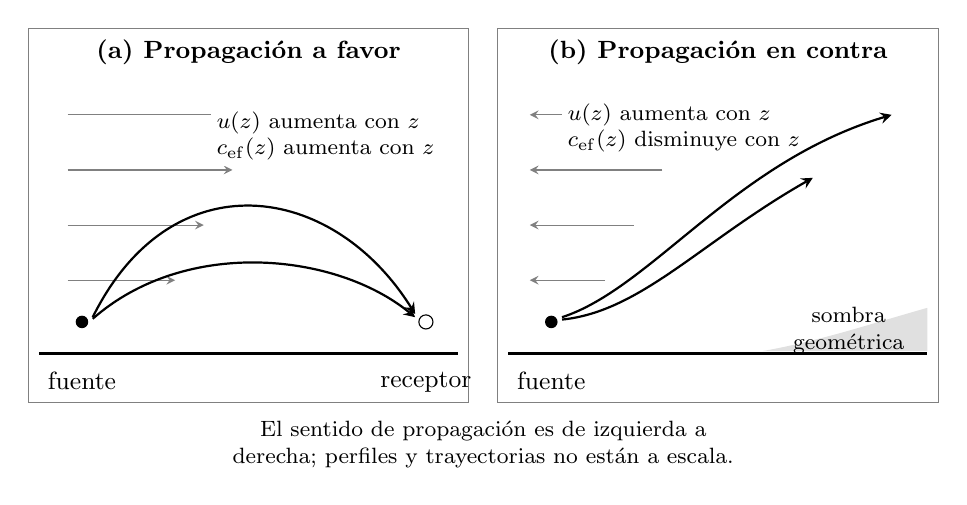
\begin{tikzpicture}[
    x=0.91cm,
    y=1cm,
    >=stealth,
    font=\small,
    rayo/.style={thick,->},
    viento/.style={gray,->},
    guia/.style={gray,dashed}
]
    % A favor
    \draw[gray] (0,0) rectangle (6.15,4.75);
    \node[font=\small\bfseries] at (3.075,4.45) {(a) Propagación a favor};
    \draw[thick] (0.15,0.62) -- (6.0,0.62);
    \node[fill=black,circle,inner sep=1.6pt] (sf) at (0.75,1.02) {};
    \node[anchor=north] at (0.75,0.50) {fuente};
    \node[draw,circle,inner sep=1.8pt] (rf) at (5.55,1.02) {};
    \node[anchor=north] at (5.55,0.50) {receptor};
    \foreach \y/\xend in {1.55/2.05,2.25/2.45,2.95/2.85,3.65/3.25}{
        \draw[viento] (0.55,\y) -- (\xend,\y);
    }
    \node[align=left,font=\footnotesize,fill=white,inner sep=2pt]
        at (4.15,3.38)
        {\(u(z)\) aumenta con \(z\)\\
         \(c_\mathrm{ef}(z)\) aumenta con \(z\)};
    \draw[rayo] (0.90,1.08)
        .. controls (2.00,3.10) and (4.25,2.80) .. (5.40,1.12);
    \draw[rayo] (0.90,1.06)
        .. controls (2.20,2.10) and (4.30,1.90) .. (5.40,1.08);

    % En contra
    \draw[gray] (6.55,0) rectangle (12.70,4.75);
    \node[font=\small\bfseries] at (9.625,4.45) {(b) Propagación en contra};
    \draw[thick] (6.70,0.62) -- (12.55,0.62);
    \node[fill=black,circle,inner sep=1.6pt] (sc) at (7.30,1.02) {};
    \node[anchor=north] at (7.30,0.50) {fuente};
    \foreach \y/\xend in {1.55/8.05,2.25/8.45,2.95/8.85,3.65/9.25}{
        \draw[viento] (\xend,\y) -- (7.00,\y);
    }
    \node[align=left,font=\footnotesize,fill=white,inner sep=2pt]
        at (9.15,3.48)
        {\(u(z)\) aumenta con \(z\)\\
         \(c_\mathrm{ef}(z)\) disminuye con \(z\)};
    \draw[rayo] (7.45,1.08)
        .. controls (8.70,1.45) and (9.85,3.05) .. (12.05,3.65);
    \draw[rayo] (7.45,1.05)
        .. controls (8.55,1.15) and (9.40,2.05) .. (10.95,2.85);
    \path[fill=black!12] (10.25,0.65) -- (12.55,0.65) -- (12.55,1.20)
        .. controls (11.70,0.98) and (11.05,0.78) .. cycle;
    \node[align=center,font=\footnotesize] at (11.45,0.91)
        {sombra\\geométrica};

    \node[font=\footnotesize,anchor=north,text width=11cm,align=center]
        at (6.35,-0.12)
        {El sentido de propagación es de izquierda a derecha; perfiles y trayectorias no están a escala.};
\end{tikzpicture}

    \caption{Refracción asociada con un gradiente de viento. Para propagación
    a favor, \(c_\mathrm{ef}\) aumenta con la altura y los rayos se curvan
    hacia el suelo; para propagación en contra, el gradiente efectivo se
    invierte y la curvatura es ascendente. Los perfiles y trayectorias son
    cualitativos.}
    \label{fig:u9-gradiente-viento}
\end{figure}

\subsection{Presión atmosférica, densidad y altitud}
\label{sec:u9-presion-altitud}

La presión atmosférica de equilibrio se representará mediante \(p_\mathrm{a}\)
y se medirá en pascales \((\text{Pa})\). La densidad de equilibrio del aire se
representará mediante \(\rho_\mathrm{a}\) y se medirá en kilogramos por metro
cúbico \((\text{kg}/\text{m}^3)\).

Para un gas ideal bajo un modelo adiabático, la velocidad puede
escribirse como~\cite{xiangBlauert2021,iso9613_1_1993}

\begin{equation}
    c=\sqrt{\frac{\gamma p_\mathrm{a}}{\rho_\mathrm{a}}},
    \label{eq:u9-velocidad-presion-densidad}
\end{equation}

donde \(\gamma\) es la razón de capacidades caloríficas y no posee unidad. Si
la composición y la temperatura se mantienen, presión y densidad cambian de
manera relacionada; por eso no corresponde atribuir a la presión aislada una
corrección universal de la velocidad.

La altitud puede modificar presión, densidad, humedad y temperatura,
pero su efecto sobre el nivel recibido depende de qué magnitud mantiene la
fuente, de la carga acústica y del receptor. No existe una corrección universal
en decibeles por cada \(1000\,\text{m}\), y esa regla no debe trasladarse a la
salida de auriculares audiométricos sin datos de calibración y del fabricante~\cite{xiangBlauert2021,iso9613_1_1993}.

\subsection{Absorción atmosférica}
\label{sec:u9-absorcion-atmosferica}

La divergencia geométrica redistribuye energía sin exigir que esta se
transforme en calor. La absorción atmosférica, en cambio, describe mecanismos
disipativos del medio.

La atenuación atmosférica depende de la frecuencia, la temperatura,
la humedad, la presión y la distancia. En general, no puede representarse
mediante una única corrección independiente de la frecuencia~\cite{xiangBlauert2021,iso9613_1_1993}. Si
\(a_\mathrm{atm}\) es un coeficiente de atenuación para una frecuencia y un
estado atmosférico definidos, expresado en decibeles por metro
\((\text{dB}/\text{m})\), una forma de organizar una estimación es

\begin{equation}
    L_{p2}
      \approx L_{p1}
      -20\log_{10}\!\left(\frac{r_2}{r_1}\right)
      -a_\mathrm{atm}(r_2-r_1).
    \label{eq:u9-distancia-absorcion-atmosferica}
\end{equation}

La ecuación separa una pérdida por divergencia de otra por absorción. El valor
de \(a_\mathrm{atm}\) no debe elegirse sin una fuente y condiciones
atmosféricas verificables.

\section{Interacción con superficies y obstáculos}
\label{sec:u9-superficies}

\subsection{Reflexión, absorción y transmisión}
\label{sec:u9-reflexion-absorcion-transmision}

Cuando una onda alcanza una partición, una parte de la energía incidente puede
regresar al primer medio, otra puede disiparse dentro del sistema y otra puede
alcanzar el segundo lado. Para separar estos resultados se utilizarán:

\begin{itemize}
    \item \(\mathcal{R}\), fracción de energía reflejada, adimensional;
    \item \(\alpha\), fracción de energía absorbida, adimensional;
    \item \(\tau\), fracción de energía transmitida, adimensional.
\end{itemize}

En un balance energético ideal, sin otras rutas, estas fracciones
cumplen~\cite{xiangBlauert2021}

\begin{equation}
    \mathcal{R}+\alpha+\tau=1.
    \label{eq:u9-balance-superficie}
\end{equation}

Los tres coeficientes dependen de la frecuencia y de las condiciones de
incidencia. Una superficie puede reducir las reflexiones dentro de un recinto
y, sin embargo, no proporcionar el aislamiento requerido entre dos espacios.
Por eso, un coeficiente de absorción alto no equivale a una pérdida por
transmisión alta.

La Figura~\ref{fig:u9-balance-superficie} organiza los tres destinos sin
confundirlos con tres instantes sucesivos: reflexión, absorción y transmisión
pueden ocurrir simultáneamente ante una misma incidencia.

\begin{figure}[htbp]
    \centering
    % Propósito: distinguir reflexión, absorción y transmisión como destinos
% simultáneos de la energía incidente.
% Origen: balance ideal R + alpha + tau = 1. Las flechas no codifican valores.
% Accesibilidad: una onda incide sobre una partición; una fracción regresa,
% otra se disipa en la partición y otra pasa al segundo recinto.
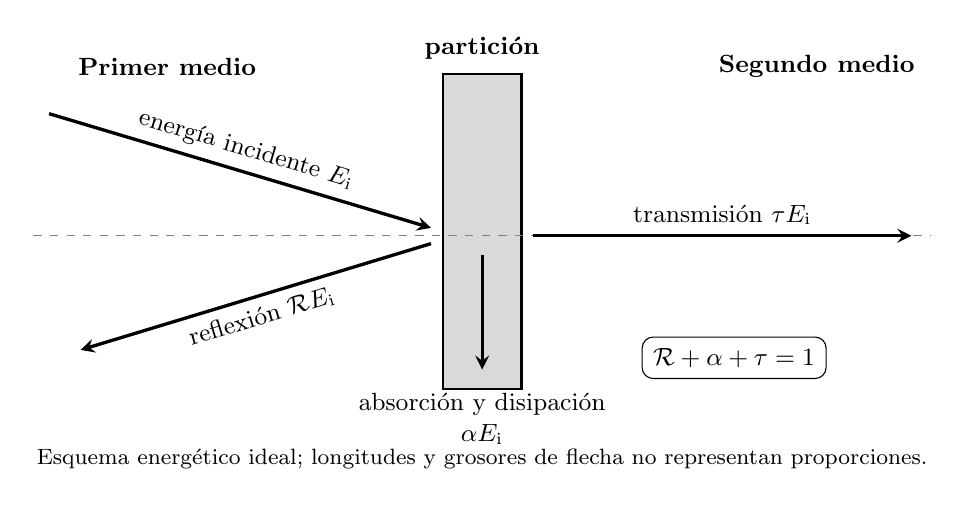
\begin{tikzpicture}[
    x=1cm,
    y=1cm,
    >=stealth,
    font=\small,
    flujo/.style={very thick,->},
    guia/.style={gray,dashed}
]
    \node[font=\small\bfseries] at (2.25,4.75) {Primer medio};
    \node[font=\small\bfseries] at (10.50,4.75) {Segundo medio};

    \path[fill=black!15] (5.75,0.65) rectangle (6.75,4.65);
    \draw[thick] (5.75,0.65) rectangle (6.75,4.65);
    \node[font=\small\bfseries,anchor=south] at (6.25,4.72) {partición};
    \draw[guia] (0.55,2.60) -- (11.95,2.60);

    \draw[flujo] (0.75,4.15) -- (5.60,2.70)
        node[midway,above,sloped] {energía incidente \(E_\mathrm{i}\)};
    \draw[flujo] (5.60,2.50) -- (1.15,1.15)
        node[midway,below,sloped] {reflexión \(\mathcal{R}E_\mathrm{i}\)};
    \draw[flujo] (6.90,2.60) -- (11.70,2.60)
        node[midway,above] {transmisión \(\tau E_\mathrm{i}\)};
    \draw[flujo] (6.25,2.35) -- (6.25,0.90);
    \node[align=center,anchor=north] at (6.25,0.72)
        {absorción y disipación\\\(\alpha E_\mathrm{i}\)};

    \node[draw,rounded corners,fill=white,inner sep=4pt]
        at (9.45,1.05) {\(\mathcal{R}+\alpha+\tau=1\)};
    \node[font=\footnotesize,anchor=north] at (6.25,0.02)
        {Esquema energético ideal; longitudes y grosores de flecha no representan proporciones.};
\end{tikzpicture}

    \caption{Balance energético ideal en una partición. Las fracciones
    reflejada \(\mathcal{R}\), absorbida \(\alpha\) y transmitida \(\tau\)
    se definen respecto de la energía incidente y, si no existen otras rutas,
    suman la unidad. El tamaño de las flechas no representa valores
    cuantitativos.}
    \label{fig:u9-balance-superficie}
\end{figure}

\subsection{Reflexión y reverberación}
\label{sec:u9-reverberacion}

Una \textbf{reflexión} es una llegada asociada con un trayecto particular. La
\textbf{reverberación} es la persistencia del campo sonoro debida a múltiples
reflexiones después de interrumpir la fuente. No toda reflexión se percibe
como un eco separado; el resultado perceptual depende además de nivel, retardo,
espectro y contexto, como se explicó en la
Sección~\ref{sec:u7-reverberacion}.

El tiempo de reverberación \(RT_{60}\), expresado en segundos
\((\text{s})\), caracteriza el intervalo necesario para que el nivel de un
campo reverberante decrezca \(60\,\text{dB}\) después de interrumpir la fuente,
medido o estimado bajo un procedimiento definido.

Para un recinto que se aproxima a las hipótesis de campo difuso y
absorción distribuida, la fórmula de Sabine en unidades métricas puede
escribirse como~\cite{moser2009,iso3382_2_2008}

\begin{equation}
    RT_{60}
      \approx
      \left(0{,}161\,\frac{\text{s}}{\text{m}}\right)\frac{V}{A},
    \qquad
    A=\sum_i \alpha_i S_i,
    \label{eq:u9-sabine}
\end{equation}

donde \(V\) es el volumen del recinto, expresado en metros cúbicos
\((\text{m}^3)\); \(S_i\) es el área de la superficie \(i\), expresada en
metros cuadrados \((\text{m}^2)\); \(\alpha_i\) es su coeficiente de absorción,
adimensional; y \(A\) es el área equivalente de absorción, expresada en metros
cuadrados \((\text{m}^2)\).

Los coeficientes y el tiempo de reverberación deben considerarse por
bandas de frecuencia. La fórmula de Sabine puede perder precisión en recintos
muy absorbentes, pequeños o con absorción distribuida de manera muy desigual~\cite{moser2009,iso3382_2_2008}.

\subsubsection*{Ejemplo resuelto: área equivalente y tiempo de reverberación}

Se considera un aula rectangular de \(8{,}0\,\text{m}\) de largo,
\(6{,}0\,\text{m}\) de ancho y \(3{,}0\,\text{m}\) de alto. Su volumen es

\[
    V=(8{,}0)(6{,}0)(3{,}0)=144\,\text{m}^3.
\]

La superficie total de piso, techo y paredes es

\[
    S_\mathrm{tot}
      =2[(8{,}0)(6{,}0)+(8{,}0)(3{,}0)+(6{,}0)(3{,}0)]
      =180\,\text{m}^2.
\]

Para una banda determinada se adopta, solo como dato didáctico, un coeficiente
medio \(\bar{\alpha}=0{,}25\). Entonces,

\[
    A=\bar{\alpha}S_\mathrm{tot}
      =(0{,}25)(180\,\text{m}^2)
      =45\,\text{m}^2,
\]

y, aplicando la ecuación~\eqref{eq:u9-sabine},

\[
    RT_{60}
      \approx
      \left(0{,}161\,\frac{\text{s}}{\text{m}}\right)
      \frac{144\,\text{m}^3}{45\,\text{m}^2}
      \approx0{,}515\,\text{s}.
\]

El resultado se redondea a \(0{,}52\,\text{s}\). No representa un valor
universal recomendado para aulas ni cabinas: solo aplica el modelo con los
datos declarados.

\subsection{Refracción}
\label{sec:u9-refraccion}

La refracción es el cambio de dirección asociado con una variación espacial de
la velocidad de propagación. En la atmósfera puede ser gradual, como en los
gradientes térmicos y de viento. En una interfaz entre medios puede acompañar
a la reflexión y a la transmisión.

Para rayos que atraviesan una interfaz ideal entre dos medios
homogéneos, una relación de Snell acústica vincula los ángulos con las
velocidades de propagación. En interfaces fluido--sólido también pueden
intervenir distintos tipos de onda y conversión modal~\cite{xiangBlauert2021}. Por este motivo, la
refracción aire--vidrio no explica por sí sola el aislamiento de una ventana
doble.

\subsection{Difracción}
\label{sec:u9-difraccion}

La difracción permite que una onda alcance regiones que no poseen línea de
vista directa con la fuente. Su importancia depende de la relación entre la
longitud de onda \(\lambda\), expresada en metros \((\text{m})\), y las
dimensiones del obstáculo o de la abertura.

La difracción suele ser más significativa cuando esas dimensiones son
comparables con \(\lambda\) o menores. Cuando el obstáculo es grande respecto
de \(\lambda\), puede formarse una región de sombra más marcada~\cite{xiangBlauert2021}. Esto explica
por qué una misma barrera puede producir resultados diferentes según la
frecuencia, pero no significa que la difracción sea transmisión a través del
material.

Por ejemplo, si \(c=343\,\text{m}/\text{s}\), para \(f=250\,\text{Hz}\) se
obtiene \(\lambda\approx1{,}37\,\text{m}\), mientras que para
\(f=4000\,\text{Hz}\) se obtiene \(\lambda\approx0{,}0858\,\text{m}\). Una
barrera de dimensiones fijas es relativamente menor frente a la primera
longitud de onda. La atenuación numérica, sin embargo, requiere conocer
alturas, distancias, ubicación del borde y un modelo de difracción.

La Figura~\ref{fig:u9-difraccion-barrera} compara dos longitudes de onda para
una misma barrera. Se representa la pérdida de línea de vista y el rodeo del
borde, pero no una transmisión a través del material.

\begin{figure}[htbp]
    \centering
    % Propósito: mostrar cómo la relación entre longitud de onda y barrera
% modifica la llegada a una zona sin línea de vista.
% Origen: comparación cualitativa para una geometría fija; no se asigna
% ninguna atenuación ni se representan datos experimentales.
% Accesibilidad: dos paneles comparan longitud de onda grande y pequeña;
% el rodeo del borde es más marcado en el primer caso.
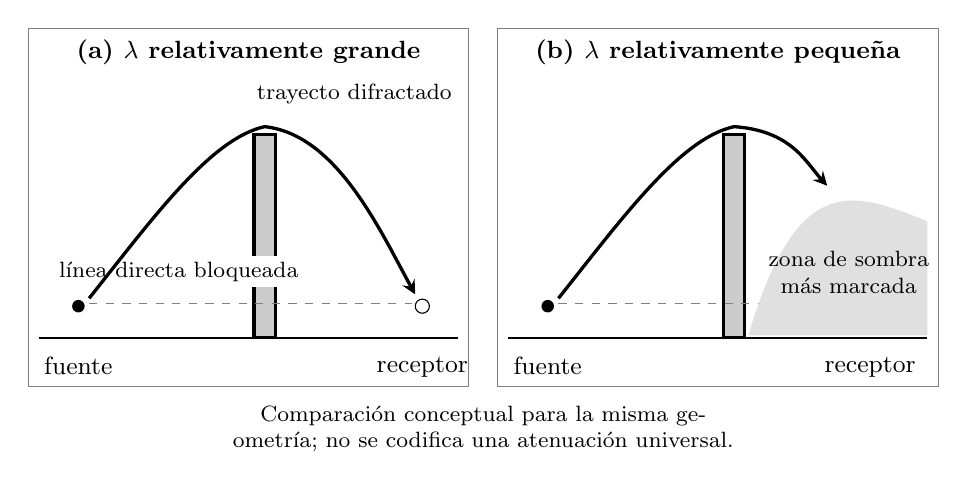
\begin{tikzpicture}[
    x=0.91cm,
    y=1cm,
    >=stealth,
    font=\small,
    camino/.style={very thick,->},
    directo/.style={gray,dashed}
]
    % Longitud de onda grande
    \draw[gray] (0,0) rectangle (6.15,4.55);
    \node[font=\small\bfseries] at (3.075,4.25)
        {(a) \(\lambda\) relativamente grande};
    \draw[thick] (0.15,0.62) -- (6.0,0.62);
    \draw[very thick,fill=black!20] (3.15,0.62) rectangle (3.45,3.20);
    \node[fill=black,circle,inner sep=1.6pt] (s1) at (0.70,1.02) {};
    \node[anchor=north] at (0.70,0.50) {fuente};
    \node[draw,circle,inner sep=1.8pt] (r1) at (5.50,1.02) {};
    \node[anchor=north] at (5.50,0.50) {receptor};
    \draw[directo] (0.85,1.05) -- (5.35,1.05);
    \node[fill=white,font=\footnotesize,inner sep=2pt]
        at (2.10,1.46) {línea directa bloqueada};
    \draw[camino] (0.85,1.12)
        .. controls (1.75,2.15) and (2.55,3.15) .. (3.30,3.30)
        .. controls (4.30,3.20) and (4.90,2.00) .. (5.40,1.17);
    \node[font=\footnotesize,fill=white,inner sep=2pt]
        at (4.55,3.72) {trayecto difractado};

    % Longitud de onda pequeña
    \draw[gray] (6.55,0) rectangle (12.70,4.55);
    \node[font=\small\bfseries] at (9.625,4.25)
        {(b) \(\lambda\) relativamente pequeña};
    \draw[thick] (6.70,0.62) -- (12.55,0.62);
    \draw[very thick,fill=black!20] (9.70,0.62) rectangle (10.00,3.20);
    \node[fill=black,circle,inner sep=1.6pt] (s2) at (7.25,1.02) {};
    \node[anchor=north] at (7.25,0.50) {fuente};
    \node[draw,circle,inner sep=1.8pt] (r2) at (11.75,1.02) {};
    \node[anchor=north] at (11.75,0.50) {receptor};
    \draw[directo] (7.40,1.05) -- (11.60,1.05);
    \draw[camino] (7.40,1.12)
        .. controls (8.30,2.15) and (9.10,3.15) .. (9.85,3.30)
        .. controls (10.65,3.25) and (10.85,2.85) .. (11.15,2.55);
    \path[fill=black!12] (10.05,0.65) -- (12.55,0.65) -- (12.55,2.10)
        .. controls (11.55,2.45) and (10.75,2.80) .. cycle;
    \node[align=center,font=\footnotesize] at (11.45,1.45)
        {zona de sombra\\más marcada};

    \node[font=\footnotesize,anchor=north,text width=11cm,align=center]
        at (6.35,-0.12)
        {Comparación conceptual para la misma geometría; no se codifica una atenuación universal.};
\end{tikzpicture}

    \caption{Difracción alrededor de una barrera. Una longitud de onda grande
    respecto del obstáculo favorece una llegada más marcada a la región sin
    línea de vista; una longitud de onda pequeña puede producir una sombra
    geométrica más definida. La figura no asigna una atenuación universal.}
    \label{fig:u9-difraccion-barrera}
\end{figure}

\section{Aislamiento, acondicionamiento e insonorización}
\label{sec:u9-aislamiento}

\subsection{Transmisión y pérdida por transmisión}
\label{sec:u9-perdida-transmision}

El coeficiente de transmisión de energía \(\tau\) es adimensional y representa
la fracción transmitida respecto de la incidente bajo condiciones definidas.
La pérdida por transmisión \(TL\), o el índice de reducción sonora
\(R\) según el contexto de medición, puede relacionarse con \(\tau\) mediante~\cite{fahyGardonio2007,iso10140_2_2021}

\begin{equation}
    R=10\log_{10}\!\left(\frac{1}{\tau}\right),
    \label{eq:u9-reduccion-transmision}
\end{equation}

donde \(R\) se expresa en decibeles \((\text{dB})\). Si
\(\tau=0{,}01\), la fracción transmitida es \(0{,}01\), es decir, uno por
ciento, y
\(R=20\,\text{dB}\) dentro de este modelo.

El valor \(R\) no es, en general, la simple diferencia entre dos niveles
medidos en cualquier par de puntos. Los procedimientos de laboratorio
y de campo establecen posiciones, áreas, bandas, campos y correcciones
específicas. Las uniones, puertas, conductos y elementos estructurales pueden
crear rutas laterales que reduzcan el aislamiento efectivo~\cite{fahyGardonio2007,iso10140_2_2021}.

\subsection{Ley de masas para una pared simple}
\label{sec:u9-ley-masas}

Una pared simple ideal ofrece mayor oposición inercial cuando aumenta su masa
por unidad de área. Se representará esa masa superficial mediante \(m\), en
kilogramos por metro cuadrado \((\text{kg}/\text{m}^2)\), y la frecuencia
mediante \(f\), en hertz \((\text{Hz})\).

Para una pared simple ideal y bajo una aproximación de incidencia difusa media, una forma didáctica habitual de la ley de masas, con \(m\) expresada en \(\text{kg}/\text{m}^2\) y \(f\) en \(\text{Hz}\), es~\cite{fahyGardonio2007}

\begin{equation}
    R_\mathrm{masa}
      \approx
      20\log_{10}\!\left[
        \left(\frac{m}{1\,\text{kg}/\text{m}^2}\right)
        \left(\frac{f}{1\,\text{Hz}}\right)
      \right]
      -47\,\text{dB},
    \label{eq:u9-ley-masas}
\end{equation}

donde \(R_\mathrm{masa}\) es una estimación de la reducción sonora, expresada
en decibeles. Las razones incluidas en el logaritmo son adimensionales.

La utilidad principal del modelo es reconocer la tendencia: al duplicar
\(m\), la estimación aumenta aproximadamente \(6{,}02\,\text{dB}\); al
duplicar \(f\), aumenta otro tanto.

La ecuación~\eqref{eq:u9-ley-masas} no describe por sí sola una pared
real. Requiere una hoja simple ideal y un intervalo alejado de resonancias,
rigidez dominante, frecuencia crítica o coincidencia, fugas y transmisión
lateral. El término constante y el campo de incidencia deben verificarse con
la fuente adoptada antes de utilizar valores absolutos~\cite{fahyGardonio2007}.

La Figura~\ref{fig:u9-ley-masas} muestra la tendencia del intervalo ideal y
separa esa predicción de las regiones en las que intervienen otros
mecanismos.

\begin{figure}[!t]
    \centering
    % Propósito: visualizar la tendencia logarítmica de la ley de masas y sus límites.
% Origen: R_masa = 20 log10(m f) + constante; duplicar m o f suma
% 20 log10(2) = 6,02 dB. No se usan datos de materiales.
% Accesibilidad: dos rectas paralelas para masas m y 2m suben con la frecuencia;
% una llave muestra 6,02 dB y se señalan regiones no descritas por el modelo.
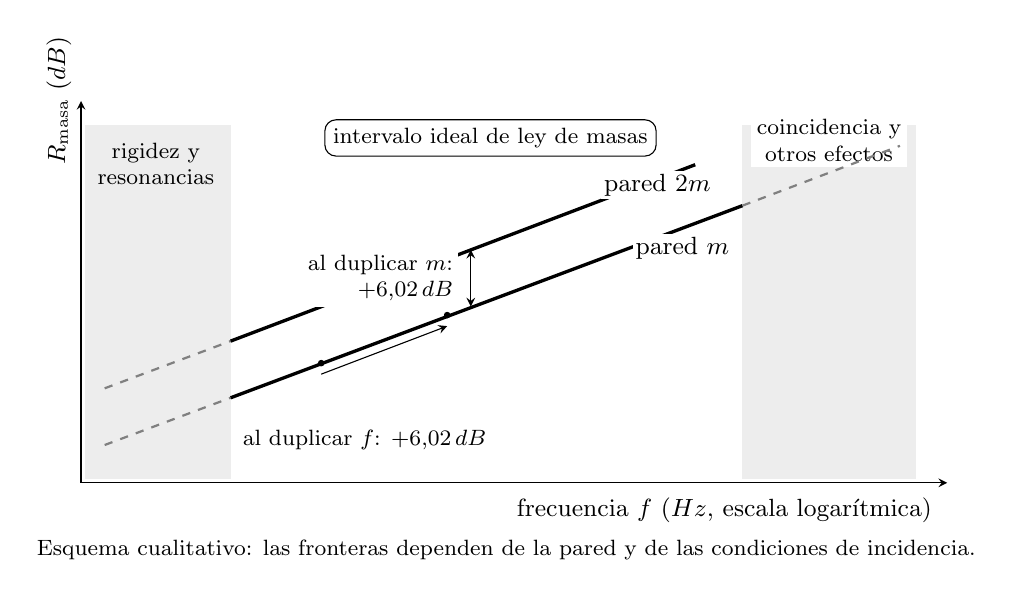
\begin{tikzpicture}[
    x=1cm,
    y=1cm,
    >=stealth,
    font=\small,
    ideal/.style={very thick},
    fuera/.style={thick,gray,dashed}
]
    \draw[->] (1.15,0.70) -- (12.15,0.70)
        node[below left=2pt,font=\small] {frecuencia \(f\) (\(\text{Hz}\), escala logarítmica)};
    \draw[->] (1.15,0.70) -- (1.15,5.55)
        node[above left,rotate=90,anchor=south,font=\small]
        {\(R_\mathrm{masa}\) (\(\text{dB}\))};

    \path[fill=black!7] (1.20,0.75) rectangle (3.05,5.25);
    \path[fill=black!7] (9.55,0.75) rectangle (11.75,5.25);
    \node[align=center,font=\footnotesize] at (2.10,4.75)
        {rigidez y\\resonancias};
    \node[align=center,font=\footnotesize,fill=white,inner sep=2pt]
        at (10.65,5.05)
        {coincidencia y\\otros efectos};

    % Pared de masa m
    \draw[fuera] (1.45,1.18) -- (3.05,1.78);
    \draw[ideal] (3.05,1.78) -- (9.55,4.22);
    \draw[fuera] (9.55,4.22) -- (11.55,4.98);
    \node[anchor=west,fill=white,inner sep=1pt] at (8.15,3.68)
        {pared \(m\)};

    % Pared de masa 2m
    \draw[fuera] (1.45,1.90) -- (3.05,2.50);
    \draw[ideal] (3.05,2.50) -- (8.95,4.74);
    \node[anchor=west,fill=white,inner sep=1pt] at (7.75,4.48)
        {pared \(2m\)};

    % Cambio por duplicar la masa, a frecuencia fija
    \draw[<->] (6.10,2.94) -- (6.10,3.66);
    \node[anchor=east,align=right,font=\footnotesize,fill=white,inner sep=2pt]
        at (5.95,3.30)
        {al duplicar \(m\):\\\(+6{,}02\,\text{dB}\)};

    % Cambio por duplicar la frecuencia sobre una misma recta
    \fill (4.20,2.22) circle (1.2pt);
    \fill (5.80,2.83) circle (1.2pt);
    \draw[->] (4.20,2.08) -- (5.80,2.69);
    \node[align=center,font=\footnotesize,fill=white,inner sep=1pt]
        at (4.75,1.25) {al duplicar \(f\): \(+6{,}02\,\text{dB}\)};

    \node[draw,rounded corners,fill=white,inner sep=3pt,font=\footnotesize]
        at (6.35,5.08) {intervalo ideal de ley de masas};
    \node[font=\footnotesize,anchor=north] at (6.55,0.10)
        {Esquema cualitativo: las fronteras dependen de la pared y de las condiciones de incidencia.};
\end{tikzpicture}

    \caption{Tendencia cualitativa de la ley de masas para una pared simple.
    En el intervalo ideal, duplicar la masa superficial \(m\) o la frecuencia
    \(f\) aumenta \(R_\mathrm{masa}\) en aproximadamente
    \(6{,}02\,\text{dB}\). Las zonas sombreadas recuerdan que resonancias,
    rigidez, coincidencia y otros efectos requieren modelos adicionales; sus
    límites no están fijados a escala.}
    \label{fig:u9-ley-masas}
\end{figure}

\subsubsection*{Ejemplo resuelto: cambio relativo según la ley de masas}

Se comparan, dentro del modelo, dos paredes simples a la misma frecuencia. La
segunda posee el doble de masa superficial:

\[
    \Delta R
      =20\log_{10}\!\left(\frac{2m}{m}\right)
      =20\log_{10}(2)
      \approx6{,}02\,\text{dB}.
\]

El resultado es una diferencia prevista por el modelo, no una especificación
constructiva. No permite determinar el aislamiento total de un recinto sin
considerar los demás elementos y rutas.

\subsection{Tres objetivos diferentes}
\label{sec:u9-acondicionamiento-insonorizacion}

\begin{description}[style=nextline]
    \item[Acondicionamiento acústico.]
    Modifica el campo dentro de un recinto mediante la distribución de
    absorción, reflexión, difusión y geometría. Puede actuar sobre el tiempo de
    reverberación y la uniformidad, pero no garantiza aislamiento exterior.

    \item[Aislamiento acústico.]
    Limita la transmisión entre espacios mediante cerramientos, uniones,
    sellos, desacoplamientos y control de rutas directas y laterales. Se evalúa
    con magnitudes y procedimientos propios.

    \item[Insonorización.]
    Se utilizará como término general para el objetivo de reducir la
    interferencia sonora en un espacio. No se tratará como una magnitud ni como
    la suma aritmética de absorción y aislamiento.
\end{description}

En un proyecto real, acondicionamiento y aislamiento pueden ser
necesarios simultáneamente, pero se dimensionan y verifican mediante criterios
diferentes~\cite{moser2009}.

\section{Cabinas audiométricas y ruido ambiente}
\label{sec:u9-cabinas}

\subsection{La cabina como sistema}
\label{sec:u9-cabina-sistema}

Una cabina sonoamortiguada no es únicamente una caja revestida con material
absorbente. Su desempeño depende del conjunto formado por paredes,
techo, piso, puerta, visor, sellos, pasacables, ventilación, uniones y apoyos
estructurales. El ruido propio de la ventilación y las rutas laterales pueden
limitar el resultado aun cuando los paneles posean una reducción sonora alta~\cite{moser2009}.

El tratamiento interior pertenece principalmente al acondicionamiento: reduce
reflexiones y ayuda a controlar el campo. La envolvente y sus conexiones
pertenecen principalmente al aislamiento: limitan la energía que ingresa desde
otros espacios. Ambos aspectos deben verificarse en la cabina terminada.

La Figura~\ref{fig:u9-cabina-sistema} permite revisar la cabina como un
conjunto de elementos conectados. Una prestación alta del panel principal no
compensa automáticamente una fuga en la puerta, un conducto sin tratamiento
o una ruta estructural.

\begin{figure}[htbp]
    \centering
    % Propósito: representar la cabina como un sistema, no como una caja revestida.
% Origen: componentes y rutas descritos en la sección; sin prestaciones
% numéricas ni especificaciones constructivas.
% Accesibilidad: corte de una cabina con envolvente, puerta, visor,
% ventilación, pasacables, tratamiento interior y tres rutas posibles de ruido.
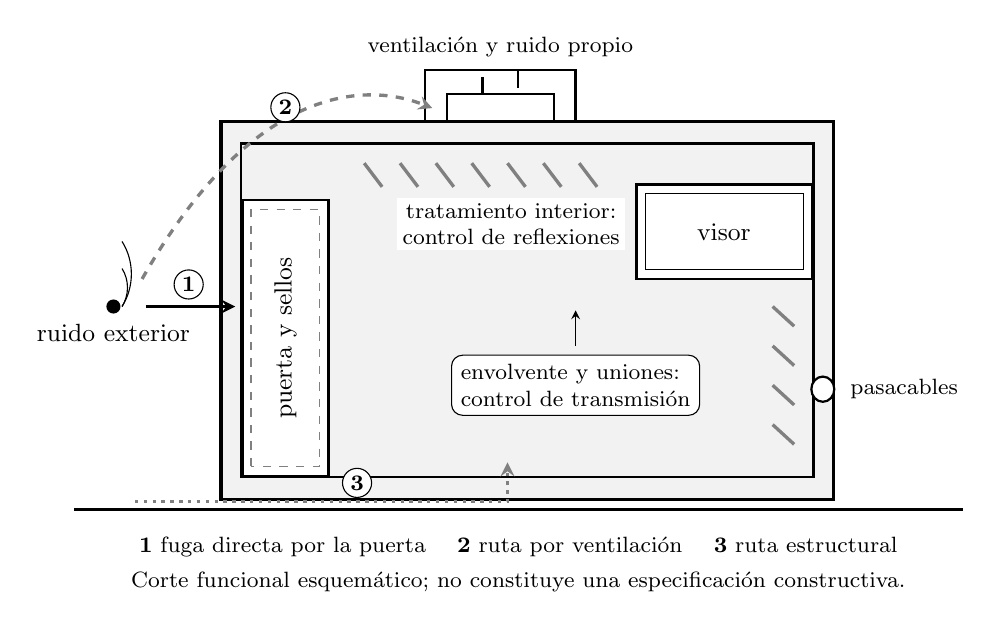
\begin{tikzpicture}[
    x=0.91cm,
    y=1cm,
    >=stealth,
    font=\small,
    directa/.style={very thick,->},
    lateral/.style={very thick,gray,dashed,->},
    estructural/.style={very thick,gray,dotted,->},
    marca/.style={draw,circle,fill=white,inner sep=1.2pt,font=\footnotesize\bfseries}
]
    % Envolvente doble y base
    \path[fill=black!5] (2.20,0.75) rectangle (10.75,5.55);
    \draw[very thick] (2.20,0.75) rectangle (10.75,5.55);
    \draw[thick] (2.48,1.03) rectangle (10.47,5.27);
    \draw[very thick] (0.15,0.62) -- (12.55,0.62);

    % Puerta y sello
    \path[fill=white] (2.50,1.05) rectangle (3.70,4.55);
    \draw[thick] (2.50,1.05) rectangle (3.70,4.55);
    \draw[gray,dashed] (2.62,1.17) rectangle (3.58,4.43);
    \node[rotate=90] at (3.10,2.80) {puerta y sellos};

    % Visor
    \path[fill=white] (8.00,3.55) rectangle (10.45,4.75);
    \draw[thick] (8.00,3.55) rectangle (10.45,4.75);
    \draw[thin] (8.12,3.67) rectangle (10.33,4.63);
    \node at (9.22,4.15) {visor};

    % Tratamiento interior
    \foreach \x in {4.20,4.70,5.20,5.70,6.20,6.70,7.20}{
        \draw[very thick,gray] (\x,5.02) -- (\x+0.25,4.72);
    }
    \foreach \y in {1.45,1.95,2.45,2.95}{
        \draw[very thick,gray] (10.20,\y) -- (9.90,\y+0.25);
    }
    \node[align=center,font=\footnotesize,fill=white,inner sep=2pt]
        at (6.25,4.25)
        {tratamiento interior:\\control de reflexiones};

    % Conducto de ventilación con dos cambios de dirección
    \draw[thick] (5.05,5.55) -- (5.05,6.20) -- (7.15,6.20) -- (7.15,5.55);
    \draw[thick] (5.35,5.55) -- (5.35,5.90) -- (6.85,5.90) -- (6.85,5.55);
    \draw[thick] (5.85,5.90) -- (5.85,6.12);
    \draw[thick] (6.35,5.98) -- (6.35,6.20);
    \node[anchor=south,font=\footnotesize] at (6.10,6.25)
        {ventilación y ruido propio};

    % Pasacables
    \draw[thick,fill=white] (10.60,2.15) circle (0.16);
    \node[anchor=west,font=\footnotesize] at (10.85,2.15) {pasacables};

    % Fuente exterior y trayectorias
    \node[fill=black,circle,inner sep=1.8pt] (s) at (0.70,3.20) {};
    \node[anchor=north] at (s.south) {ruido exterior};
    \draw (0.82,3.20) arc (-35:35:0.42);
    \draw (0.82,3.20) arc (-35:35:0.72);

    \draw[directa] (1.15,3.20) -- (2.40,3.20);
    \node[marca] at (1.75,3.48) {1};
    \draw[lateral] (1.10,3.55)
        .. controls (2.60,5.95) and (4.15,6.08) .. (5.15,5.72);
    \node[marca] at (3.10,5.73) {2};
    \draw[estructural] (1.00,0.72) -- (6.20,0.72) -- (6.20,1.22);
    \node[marca] at (4.10,0.96) {3};

    \node[draw,rounded corners,fill=white,align=left,font=\footnotesize]
        at (7.15,2.20)
        {envolvente y uniones:\\control de transmisión};
    \draw[->] (7.15,2.70) -- (7.15,3.15);

    \node[font=\footnotesize,anchor=north,text width=11cm,align=center]
        at (6.35,0.40)
        {\textbf{1} fuga directa por la puerta \quad
         \textbf{2} ruta por ventilación \quad
         \textbf{3} ruta estructural};
    \node[font=\footnotesize,anchor=north] at (6.35,-0.05)
        {Corte funcional esquemático; no constituye una especificación constructiva.};
\end{tikzpicture}

    \caption{Corte funcional de una cabina sonoamortiguada. La envolvente,
    las uniones, la puerta, el visor, la ventilación y los pasajes de servicio
    intervienen en el aislamiento; el tratamiento interior controla
    principalmente las reflexiones. Las rutas señaladas son posibles caminos
    de ingreso de ruido y no representan una especificación constructiva.}
    \label{fig:u9-cabina-sistema}
\end{figure}

\subsection{Ruido ambiente máximo permitido}
\label{sec:u9-ruido-cabina}

No corresponde asignar a toda cabina un límite único en
\(\text{dB(A)}\). Los niveles máximos admisibles para una audiometría
dependen, entre otros factores, de la vía de prueba, el transductor, su
atenuación, las bandas de frecuencia evaluadas y el menor nivel de audición
que se pretende medir~\cite{iso8253_1_2010,ansiS31_2023,iso8253_2_2009}.

Una futura tabla normativa deberá declarar como mínimo:

\begin{itemize}
    \item norma, edición y jurisdicción o adopción aplicable;
    \item procedimiento audiométrico y vía de presentación;
    \item tipo de transductor o condición de campo sonoro;
    \item bandas de frecuencia y descriptor de nivel utilizados;
    \item menor nivel de audición que se desea medir sin enmascaramiento
    ambiental significativo;
    \item instrumentación, posición y condiciones de medición.
\end{itemize}

La aptitud de una cabina debe demostrarse mediante mediciones por
bandas y un procedimiento compatible con la audiometría prevista. Una lectura
ponderada A obtenida con una aplicación telefónica no reemplaza esa
verificación~\cite{iso8253_1_2010,ansiS31_2023,iso8253_2_2009}.

\section{Relación con Fonoaudiología}
\label{sec:u9-fonoaudiologia}

Los conceptos de esta unidad permiten formular preguntas físicas antes de una
medición o de una intervención:

\begin{itemize}
    \item en audiometría de campo sonoro, identificar el punto de referencia,
    la geometría, la directividad y las reflexiones evita confundir un cambio
    de posición con un cambio del estímulo programado;
    \item en una cabina, separar acondicionamiento y aislamiento permite
    distinguir reflexiones interiores de ruido que ingresa desde el exterior;
    \item en una evaluación ambiental, registrar estado atmosférico, distancia,
    altura y dirección ayuda a interpretar por qué dos mediciones no son
    directamente comparables;
    \item al estudiar una barrera o un cerramiento, diferenciar difracción,
    transmisión y rutas laterales evita atribuir todo el resultado al material
    principal.
\end{itemize}

Los procedimientos audiométricos, la aceptación normativa de una
cabina y el diseño constructivo requieren fuentes vigentes, instrumentación
adecuada y personal competente. Esta unidad no reemplaza esos procedimientos~\cite{iso8253_1_2010,ansiS31_2023,iso8253_2_2009}.

\section{Errores frecuentes}
\label{sec:u9-errores}

\begin{description}[style=nextline]
    \item[``Duplicar la distancia siempre resta \(6\,\text{dB}\)''.]
    La regla requiere campo aproximadamente libre, campo lejano, misma
    dirección y pérdidas adicionales despreciables.

    \item[``El viento a favor aumenta necesariamente el nivel''.]
    Un viento uniforme modifica el tiempo de propagación; los cambios de nivel
    a distancia requieren considerar gradientes, turbulencia, suelo y
    geometría.

    \item[``La altitud resta una cantidad fija de decibeles''.]
    No existe una corrección universal independiente de la fuente, el receptor
    y el estado atmosférico.

    \item[``Absorber es aislar''.]
    La absorción reduce la energía que regresa al recinto; el aislamiento
    limita la energía que atraviesa el sistema hacia otro espacio.

    \item[``Una reflexión es reverberación''.]
    Una reflexión corresponde a un trayecto; la reverberación surge de la
    persistencia producida por muchas reflexiones.

    \item[``Los graves atraviesan una pared por difracción''.]
    La difracción alrededor de bordes y la transmisión a través de un
    cerramiento son mecanismos distintos.

    \item[``La ley de masas predice cualquier pared''.]
    Es un modelo aproximado para una hoja simple y no incluye automáticamente
    resonancias, coincidencia, sistemas dobles, fugas o rutas laterales.

    \item[``Un valor bajo en \(\text{dB(A)}\) certifica una cabina''.]
    La aptitud audiométrica exige criterios por bandas y condiciones de prueba
    definidas.
\end{description}

\section{Síntesis}
\label{sec:u9-sintesis}

El nivel recibido no pertenece solamente a la fuente: resulta de la emisión,
la directividad, el trayecto y la posición de medición. La ley del cuadrado
inverso describe divergencia geométrica bajo condiciones ideales; la absorción
atmosférica representa una pérdida adicional dependiente de la frecuencia y
del estado del aire.

La temperatura y el viento uniformes modifican velocidades y tiempos de
propagación. Sus gradientes pueden refractar los trayectos. La presión y la
densidad deben analizarse de manera conjunta, por lo que la altitud no produce
una corrección universal de nivel.

En una superficie, reflexión, absorción y transmisión describen destinos
diferentes de la energía. La reverberación resulta de reflexiones sucesivas;
la difracción permite alcanzar regiones sin línea de vista; y la transmisión
a través de una pared no debe confundirse con la difracción alrededor de ella.

El acondicionamiento controla el campo interior y el aislamiento limita el
paso entre espacios. La ley de masas aporta una tendencia para paredes simples,
pero una cabina real depende de todos sus elementos y rutas. Su aptitud para
audiometría solo puede establecerse con criterios normativos verificables y
compatibles con la prueba prevista.

\section{Ejercicios y autoevaluación}
\label{sec:u9-ejercicios}

\subsection*{Preguntas conceptuales}

\begin{enumerate}[label=\textbf{C\arabic*.},leftmargin=*]
    \item Distinga nivel de potencia acústica de una fuente y nivel de presión
    sonora recibido en un punto.
    \item Explique por qué la pérdida por divergencia geométrica no es
    absorción atmosférica.
    \item Compare viento uniforme y gradiente de viento respecto de sus
    posibles efectos sobre tiempo de llegada y trayectoria.
    \item Explique por qué una inversión térmica puede modificar el alcance sin
    cambiar la frecuencia emitida por la fuente.
    \item Distinga reflexión, reverberación y eco.
    \item Distinga absorción material, transmisión y aislamiento.
    \item Explique por qué la difracción alrededor de una barrera no es
    transmisión a través de una pared.
    \item Compare acondicionamiento e insonorización con aislamiento acústico.
    \item Indique dos limitaciones de la ley de masas.
    \item Explique por qué un único valor en \(\text{dB(A)}\) no basta para
    certificar una cabina audiométrica.
\end{enumerate}

\subsection*{Identificación e interpretación de gráficos}

\begin{enumerate}[label=\textbf{V\arabic*.},leftmargin=*]
    \item Observe las Figuras~\ref{fig:u4-propagacion-esferica} y
    \ref{fig:u4-directividad-q}.
    \begin{enumerate}
        \item Identifique cuál representa divergencia geométrica y cuál
        representa redistribución direccional de la potencia.
        \item Explique qué comparación debe mantenerse para atribuir una
        diferencia de nivel a la directividad.
        \item Indique si corresponde sumar \(DI\) a un nivel que ya fue medido
        en la dirección representada.
    \end{enumerate}

    \item Compare las Figuras~\ref{fig:u9-gradientes-termicos} y
    \ref{fig:u9-gradiente-viento}.
    \begin{enumerate}
        \item Para cada panel, identifique la región de menor velocidad
        \(c\), o de menor velocidad efectiva \(c_\mathrm{ef}\), hacia la que
        se curvan los trayectos.
        \item Localice las regiones de sombra geométrica.
        \item Explique por qué los esquemas no permiten predecir una
        corrección universal de nivel en decibeles ni un cambio de la
        frecuencia emitida.
    \end{enumerate}

    \item En la Figura~\ref{fig:u9-balance-superficie}:
    \begin{enumerate}
        \item asocie cada flecha con energía incidente, reflejada, absorbida o
        transmitida;
        \item escriba el balance ideal entre
        \(\mathcal{R}\), \(\alpha\) y \(\tau\);
        \item explique por qué el dibujo no autoriza a estimar valores
        numéricos a partir de la longitud de las flechas.
    \end{enumerate}

    \item Compare los dos paneles de la
    Figura~\ref{fig:u9-difraccion-barrera}. Indique en cuál se espera una
    llegada relativamente mayor a la región sin línea de vista y qué
    información geométrica faltaría para calcular una atenuación.

    \item En la Figura~\ref{fig:u9-ley-masas}, identifique:
    \begin{enumerate}
        \item el cambio vertical previsto al duplicar la masa superficial
        \(m\), expresada en \(\text{kg}/\text{m}^2\);
        \item el cambio previsto al duplicar la frecuencia \(f\), expresada
        en \(\text{Hz}\);
        \item las regiones donde la recta ideal deja de ser una descripción
        suficiente.
    \end{enumerate}

    \item Use la Figura~\ref{fig:u9-cabina-sistema} para:
    \begin{enumerate}
        \item identificar las tres rutas de ingreso señaladas;
        \item separar los elementos que controlan principalmente transmisión
        de los que controlan principalmente reflexiones interiores;
        \item justificar por qué el desempeño del panel principal no basta
        para predecir el ruido ambiente dentro de la cabina.
    \end{enumerate}
\end{enumerate}

\subsection*{Ejercicios numéricos guiados}

\begin{enumerate}[label=\textbf{G\arabic*.},leftmargin=*]
    \item En campo aproximadamente libre se miden \(82\,\text{dB SPL}\) a
    \(r_1=1{,}5\,\text{m}\). Para estimar el nivel a
    \(r_2=6{,}0\,\text{m}\):
    \begin{enumerate}
        \item calcule la razón adimensional \(r_2/r_1\);
        \item calcule el cambio de nivel debido a divergencia;
        \item obtenga \(L_{p2}\), expresado en \(\text{dB SPL}\), y declare
        las hipótesis utilizadas.
    \end{enumerate}

    \item Para un factor de directividad adimensional \(Q=8\):
    \begin{enumerate}
        \item escriba la relación entre \(DI\) y \(Q\);
        \item calcule \(DI\), expresado en decibeles \((\text{dB})\);
        \item explique qué se compara y por qué el resultado no implica
        creación de energía.
    \end{enumerate}

    \item Use la ecuación~\eqref{eq:u9-velocidad-temperatura} para estimar
    \(c\), expresada en \(\text{m}/\text{s}\), a
    \(5\,^{\circ}\text{C}\) y a \(25\,^{\circ}\text{C}\). Luego, para una
    fuente que emite un tono de \(f=1000\,\text{Hz}\):
    \begin{enumerate}
        \item calcule la longitud de onda \(\lambda\), expresada en metros
        \((\text{m})\), en ambos casos;
        \item indique qué magnitud cambia y cuál conserva el valor fijado por
        la fuente.
    \end{enumerate}

    \item Una superficie ideal presenta las fracciones adimensionales
    \(\mathcal{R}=0{,}55\) y \(\alpha=0{,}30\).
    \begin{enumerate}
        \item Use la ecuación~\eqref{eq:u9-balance-superficie} para hallar la
        fracción transmitida \(\tau\).
        \item Exprese \(\tau\) también como porcentaje de la energía
        incidente.
    \end{enumerate}

    \item Dentro del modelo de transmisión, para una fracción adimensional
    \(\tau=0{,}001\):
    \begin{enumerate}
        \item calcule \(1/\tau\);
        \item calcule \(R\), expresado en decibeles \((\text{dB})\);
        \item interprete \(\tau\) como porcentaje de la energía incidente.
    \end{enumerate}
\end{enumerate}

\subsection*{Ejercicios numéricos autónomos}

\begin{enumerate}[label=\textbf{A\arabic*.},leftmargin=*]
    \item Un nivel recibido es \(76\,\text{dB SPL}\) a
    \(r_1=2{,}0\,\text{m}\). Estime el nivel a \(r_2=10{,}0\,\text{m}\) bajo
    las hipótesis de la ecuación~\eqref{eq:u9-distancia}.

    \item Para \(c=343\,\text{m}/\text{s}\), calcule \(\lambda\) a
    \(125\,\text{Hz}\), \(500\,\text{Hz}\) y \(4000\,\text{Hz}\). Ordene las
    frecuencias según la importancia esperable de la difracción para una misma
    barrera, sin asignar una atenuación numérica.

    \item Un recinto rectangular mide \(5{,}0\,\text{m}\) por
    \(4{,}0\,\text{m}\) por \(3{,}0\,\text{m}\). Para una banda determinada se
    adopta el coeficiente medio adimensional
    \(\bar{\alpha}=0{,}20\) en todas las superficies. Calcule
    \(S_\mathrm{tot}\), expresada en \(\text{m}^2\); \(A\), expresada en
    \(\text{m}^2\); y \(RT_{60}\), expresado en segundos \((\text{s})\),
    mediante Sabine. Declare las limitaciones del resultado.

    \item Según la tendencia ideal de la ley de masas, estime el cambio de
    \(R_\mathrm{masa}\), expresado en decibeles \((\text{dB})\), si
    \(m_2=2m_1\), con \(m_1\) y \(m_2\) expresadas en
    \(\text{kg}/\text{m}^2\), y simultáneamente \(f_2=2f_1\), con \(f_1\) y
    \(f_2\) expresadas en \(\text{Hz}\).
\end{enumerate}

\subsection*{Aplicaciones a Fonoaudiología}

\begin{enumerate}[label=\textbf{F\arabic*.},leftmargin=*]
    \item En una audiometría de campo sonoro se obtienen niveles diferentes en
    dos posiciones separadas dentro de la zona de prueba. Proponga una
    secuencia de comprobaciones que incluya fuente, trayecto y receptor.

    \item En una cabina se reduce la reverberación al agregar absorbentes, pero
    continúa ingresando ruido de un pasillo. Explique por qué el resultado no
    es contradictorio y qué rutas deberían inspeccionarse.

    \item Una medición exterior cambia entre la tarde y la noche sin que la
    fuente industrial haya modificado su operación. Proponga variables
    atmosféricas y geométricas que deberían registrarse antes de atribuir la
    diferencia a la fuente.

    \item Se informa que una pared posee una reducción alta, pero el nivel
    interior continúa dominado por bajas frecuencias. Mencione al menos cuatro
    explicaciones que no contradigan necesariamente el dato del panel.

    \item Una aplicación telefónica informa \(28\,\text{dB(A)}\) dentro de una
    cabina. Explique qué datos faltan para decidir si la cabina es apta para
    audiometría tonal por una vía y un transductor determinados.
\end{enumerate}

\subsection*{Pregunta integradora}

\begin{enumerate}[label=\textbf{I\arabic*.},leftmargin=*]
    \item Una clínica proyecta ubicar una cabina próxima a una avenida. Organice
    un análisis en las etapas fuente--trayecto--receptor. Incluya espectro y
    directividad de las fuentes, propagación exterior, transmisión por la
    envolvente, rutas laterales, acondicionamiento interior y verificación del
    ruido ambiente. Indique qué partes pueden estimarse con los modelos de esta
    unidad y cuáles requieren medición, norma o diseño especializado.
\end{enumerate}

\subsection*{Errores frecuentes y distractores razonables}

Para cada afirmación, indique si es correcta, incorrecta o incompleta y
justifique.

\begin{enumerate}[label=\textbf{D\arabic*.},leftmargin=*]
    \item ``Si una pared tiene el coeficiente de absorción adimensional
    \(\alpha=0{,}90\), bloquea el noventa por ciento del sonido que intenta
    atravesarla''.
    \item ``A favor del viento siempre deben sumarse decibeles al nivel
    calculado por distancia''.
    \item ``Una cabina con poco \(RT_{60}\) es automáticamente apta para
    audiometría''.
    \item ``Si una fuente con el factor de directividad adimensional \(Q=4\)
    produce \(80\,\text{dB SPL}\) medidos en una dirección, corresponde sumar
    nuevamente \(6\,\text{dB}\) por directividad''.
    \item ``Si aumenta la temperatura uniforme del aire, aumentan
    necesariamente la frecuencia recibida y la altura tonal percibida''.
\end{enumerate}

\section{Soluciones y orientaciones}
\label{sec:u9-soluciones}

\subsection*{Preguntas conceptuales}

\begin{enumerate}[label=\textbf{C\arabic*.},leftmargin=*]
    \item \(L_W\) describe la emisión total de la fuente mediante una potencia
    de referencia; \(L_p\) describe presión acústica en un punto y depende
    también del trayecto y la posición.
    \item La divergencia redistribuye energía sobre un área creciente. La
    absorción atmosférica transforma parte de la energía mecánica mediante
    procesos disipativos y depende del estado del aire y de la frecuencia.
    \item El viento uniforme modifica principalmente la velocidad respecto del
    suelo y el tiempo de llegada. Un gradiente modifica la velocidad efectiva
    con la altura y puede curvar el trayecto.
    \item La fuente fija la frecuencia. El gradiente modifica \(c\) con la
    altura y refracta el trayecto; si \(f\) se conserva, cambia
    \(\lambda=c/f\), no la frecuencia emitida.
    \item Una reflexión corresponde a una llegada por un trayecto. La
    reverberación es la persistencia de múltiples reflexiones. Un eco es una
    interpretación perceptual posible de una llegada separada.
    \item Absorción es disipación dentro del sistema; transmisión es la fracción
    que alcanza el otro lado; aislamiento es el desempeño del conjunto para
    limitar el paso entre espacios.
    \item La difracción redistribuye la onda alrededor de bordes o aberturas.
    La transmisión describe energía que atraviesa un cerramiento.
    \item El acondicionamiento modifica el campo interior. El aislamiento limita
    el paso entre espacios. Insonorización se usa como objetivo general y no
    como una magnitud que sume ambos efectos.
    \item Entre las limitaciones posibles están resonancias, coincidencia,
    rigidez, sistemas multicapa, fugas y transmisión lateral.
    \item La ponderación A combina frecuencias en un único descriptor. La
    audiometría exige comprobar bandas, vía, transductor, atenuación y menor
    nivel que se desea medir.
\end{enumerate}

\subsection*{Identificación e interpretación de gráficos}

\begin{enumerate}[label=\textbf{V\arabic*.},leftmargin=*]
    \item La Figura~\ref{fig:u4-propagacion-esferica} representa la
    redistribución geométrica de la energía al aumentar la distancia. La
    Figura~\ref{fig:u4-directividad-q} representa cómo una fuente distribuye
    su potencia entre direcciones. Para comparar directividad deben mantenerse
    la potencia acústica total, la distancia, el medio y las demás condiciones
    relevantes. Si \(L_p\) ya fue medido en una dirección, no corresponde
    volver a sumarle \(DI\).

    \item En la Figura~\ref{fig:u9-gradientes-termicos}, los trayectos se
    curvan hacia las regiones rotuladas con menor \(c\): hacia arriba cuando
    la velocidad es mayor cerca del suelo y hacia abajo en el perfil
    invertido. En la Figura~\ref{fig:u9-gradiente-viento}, la propagación a
    favor presenta menor \(c_\mathrm{ef}\) cerca del suelo y curvatura
    descendente; en contra, el gradiente efectivo produce curvatura
    ascendente. Las sombras aparecen cerca del suelo cuando los trayectos se
    apartan de esa región. Como no se especifican perfiles, distancias,
    turbulencia ni interacción con el suelo, no puede deducirse una corrección
    universal de nivel. La fuente sigue fijando la frecuencia emitida.

    \item La flecha que llega a la partición representa la energía incidente;
    las flechas que regresan, se disipan en la partición y llegan al segundo
    medio representan, respectivamente, reflexión, absorción y transmisión.
    El balance ideal es
    \(\mathcal{R}+\alpha+\tau=1\). Las longitudes y los grosores de las flechas
    son esquemáticos, por lo que no codifican las fracciones numéricas.

    \item En el panel de longitud de onda relativamente grande se espera una
    llegada relativamente mayor a la zona sin línea de vista. Para calcular
    una atenuación se requieren, como mínimo, la longitud de onda, la altura y
    forma de la barrera, las posiciones y alturas de fuente y receptor, y las
    distancias al borde. La figura no proporciona esos datos.

    \item En el intervalo ideal, la separación entre las rectas muestra que
    duplicar \(m\) aumenta \(R_\mathrm{masa}\) aproximadamente
    \(6{,}02\,\text{dB}\). Avanzar una duplicación de frecuencia sobre una
    misma recta produce el mismo cambio. Las zonas sombreadas indican regiones
    donde rigidez, resonancias, coincidencia u otros mecanismos impiden usar
    la recta ideal como descripción suficiente.

    \item Las rutas numeradas corresponden al ingreso directo por puerta,
    al conducto de ventilación y a la transmisión estructural. La envolvente,
    las uniones, la puerta, el visor, los pasacables y la ventilación
    intervienen principalmente en el control de transmisión; el tratamiento
    interior controla principalmente las reflexiones. Un panel principal de
    buen desempeño no elimina fugas ni rutas laterales y, por eso, no
    determina por sí solo el ruido ambiente interior.
\end{enumerate}

\subsection*{Ejercicios numéricos guiados}

\begin{enumerate}[label=\textbf{G\arabic*.},leftmargin=*]
    \item La razón es \(r_2/r_1=6{,}0/1{,}5=4\). Entonces,
    \[
        L_{p2}=82-20\log_{10}(4)
        \approx82-12{,}04
        \approx69{,}96\,\text{dB SPL}.
    \]
    Redondeado al decibel, se obtienen \(70\,\text{dB SPL}\). Se suponen campo
    lejano, misma dirección, fuente estable, medio uniforme, reflexiones y
    pérdidas adicionales despreciables.

    \item
    \[
        DI=10\log_{10}(8)\approx9{,}03\,\text{dB}.
    \]
    Se compara el nivel en una dirección con el de una fuente omnidireccional
    de igual potencia y a igual distancia. El resultado describe
    redistribución direccional de la potencia y no creación de energía.

    \item
    \[
        c_5\approx331+0{,}6(5)=334\,\text{m}/\text{s},
        \qquad
        c_{25}\approx331+0{,}6(25)=346\,\text{m}/\text{s}.
    \]
    Para \(f=1000\,\text{Hz}\),
    \[
        \lambda_5=\frac{334}{1000}=0{,}334\,\text{m},
        \qquad
        \lambda_{25}=\frac{346}{1000}=0{,}346\,\text{m}.
    \]
    Cambian \(c\) y \(\lambda\). En el modelo considerado, la frecuencia
    conserva el valor \(f=1000\,\text{Hz}\) fijado por la fuente.

    \item
    \[
        \tau=1-\mathcal{R}-\alpha
        =1-0{,}55-0{,}30
        =0{,}15.
    \]
    Dentro del balance ideal, se transmite el quince por ciento de la energía
    incidente.

    \item
    \[
        \frac{1}{\tau}=\frac{1}{0{,}001}=1000,
        \qquad
        R=10\log_{10}\!\left(\frac{1}{0{,}001}\right)
        =10\log_{10}(1000)
        =30\,\text{dB}.
    \]
    La fracción transmitida es \(0{,}001\), es decir, una décima de uno por
    ciento.
\end{enumerate}

\subsection*{Ejercicios numéricos autónomos}

\begin{enumerate}[label=\textbf{A\arabic*.},leftmargin=*]
    \item
    \[
        L_{p2}
          =76-20\log_{10}\!\left(\frac{10{,}0}{2{,}0}\right)
          \approx76-13{,}98
          \approx62{,}02\,\text{dB SPL}.
    \]
    El resultado es aproximadamente \(62\,\text{dB SPL}\) bajo las hipótesis
    del modelo.

    \item
    \[
        \begin{aligned}
            \lambda_{125}
              &=\frac{343}{125}\approx2{,}74\,\text{m},
            &
            \lambda_{500}
              &=\frac{343}{500}\approx0{,}686\,\text{m},\\
            \lambda_{4000}
              &=\frac{343}{4000}\approx0{,}0858\,\text{m}.
        \end{aligned}
    \]
    Para una misma barrera, se espera mayor importancia relativa de la
    difracción a \(125\,\text{Hz}\), luego a \(500\,\text{Hz}\) y finalmente a
    \(4000\,\text{Hz}\). No puede asignarse una atenuación sin geometría.

    \item El volumen es
    \(V=(5{,}0)(4{,}0)(3{,}0)=60\,\text{m}^3\). La superficie total es
    \[
        S_\mathrm{tot}
          =2[(5{,}0)(4{,}0)+(5{,}0)(3{,}0)+(4{,}0)(3{,}0)]
          =94\,\text{m}^2.
    \]
    Por lo tanto,
    \[
        A=(0{,}20)(94\,\text{m}^2)=18{,}8\,\text{m}^2,
    \]
    y
    \[
        RT_{60}
          \approx
          \left(0{,}161\,\frac{\text{s}}{\text{m}}\right)
          \frac{60\,\text{m}^3}{18{,}8\,\text{m}^2}
          \approx0{,}514\,\text{s}.
    \]
    El resultado es \(0{,}51\,\text{s}\) para la banda y los supuestos
    declarados; no constituye un requisito universal.

    \item Duplicar la masa aporta aproximadamente \(6{,}02\,\text{dB}\) y
    duplicar la frecuencia otros \(6{,}02\,\text{dB}\). El cambio combinado es
    aproximadamente \(12{,}04\,\text{dB}\) dentro del modelo ideal.
\end{enumerate}

\subsection*{Aplicaciones a Fonoaudiología}

\begin{enumerate}[label=\textbf{F\arabic*.},leftmargin=*]
    \item Conviene comprobar estabilidad y orientación de la fuente, frecuencia
    y patrón de radiación, distancias y alturas, reflexiones próximas,
    posiciones del micrófono y procedimiento de verificación. La diferencia no
    debe atribuirse automáticamente al audiómetro.
    \item Los absorbentes actúan sobre reflexiones interiores; el ruido del
    pasillo puede ingresar por puerta, sellos, visor, ventilación, uniones,
    estructura o pasacables. Deben inspeccionarse rutas directas y laterales.
    \item Deben registrarse temperatura y su perfil, viento y dirección,
    humedad, presión, distancia, alturas, estado del suelo, obstáculos y
    ubicación de fuente y receptor.
    \item Son posibles una banda fuera del mejor desempeño del panel,
    resonancias o coincidencia, puerta o visor más débiles, fugas, ventilación,
    uniones rígidas y transmisión lateral estructural.
    \item Faltan, como mínimo, calibración e incertidumbre del instrumento,
    niveles por bandas, vía, transductor, atenuación del transductor, menor
    nivel de prueba, posición de medición y norma vigente aplicable.
\end{enumerate}

\subsection*{Pregunta integradora}

\begin{enumerate}[label=\textbf{I\arabic*.},leftmargin=*]
    \item El análisis debe caracterizar primero las fuentes de la avenida y su
    espectro; luego distancia, directividad, atmósfera, suelo y barreras; después
    la transmisión por cada elemento y por rutas laterales; y finalmente el
    campo y el ruido interior en los puntos de ensayo. La divergencia, cambios
    relativos de directividad, balance energético, Sabine y tendencia de la ley
    de masas permiten estimaciones iniciales. Los valores de aceptación, el
    diseño de la envolvente y la certificación requieren mediciones,
    procedimientos normativos y diseño especializado.
\end{enumerate}

\subsection*{Errores frecuentes y distractores razonables}

\begin{enumerate}[label=\textbf{D\arabic*.},leftmargin=*]
    \item Incorrecta. \(\alpha\) describe absorción bajo condiciones definidas,
    no la fracción bloqueada entre dos recintos. Para transmisión se necesita
    \(\tau\) o una magnitud de reducción sonora.
    \item Incorrecta. No existe una suma universal. Deben considerarse perfil
    de viento, refracción, turbulencia, suelo y geometría.
    \item Incorrecta. Un \(RT_{60}\) pequeño describe el campo interior, pero no
    demuestra que el ruido ambiente cumpla los requisitos audiométricos.
    \item Incorrecta. Si los \(80\,\text{dB SPL}\) ya fueron medidos en esa
    dirección, la directividad ya forma parte del resultado.
    \item Incorrecta. En una atmósfera uniforme y sin movimiento relativo
    entre fuente y receptor, la fuente fija la frecuencia. El cambio de
    velocidad de propagación modifica la longitud de onda
    \(\lambda=c/f\), pero no permite afirmar por sí solo un cambio de
    frecuencia ni de altura tonal.
\end{enumerate}

\section{Glosario}
\label{sec:u9-glosario}

\begin{description}[style=nextline]
    \item[Acondicionamiento acústico.]
    Intervención sobre el campo sonoro dentro de un recinto.

    \item[Área equivalente de absorción (\(A\)).]
    Suma de los productos entre área y coeficiente de absorción; se expresa en
    metros cuadrados \((\text{m}^2)\).

    \item[Difracción.]
    Redistribución de una onda alrededor de bordes o a través de aberturas,
    dependiente de la relación entre longitud de onda y geometría.

    \item[Gradiente.]
    Variación espacial de una magnitud, como temperatura o velocidad del
    viento.

    \item[Índice de directividad (\(DI\)).]
    Expresión en decibeles del factor de directividad:
    \(DI=10\log_{10}Q\).

    \item[Insonorización.]
    Objetivo general de reducir interferencia sonora; no constituye una
    magnitud física única.

    \item[Pérdida por transmisión.]
    Descriptor en decibeles relacionado con la fracción de energía transmitida
    por una partición bajo condiciones definidas.

    \item[Refracción.]
    Cambio de dirección de propagación asociado con una variación espacial de
    la velocidad.

    \item[Reverberación.]
    Persistencia del campo sonoro producida por múltiples reflexiones después
    de interrumpir una fuente.

    \item[Transmisión.]
    Paso de energía acústica desde un lado de un sistema hacia el otro.
\end{description}

\section{Fuentes externas y alcance documental}
\label{sec:u9-fuentes}

La revisión bibliográfica evaluó las 24 afirmaciones atmosféricas,
constructivas, audiométricas y normativas que estaban marcadas con
\verb|\verify{...}|. Todas quedaron respaldadas con textos académicos,
artículos revisados por pares, normas técnicas vigentes o documentación
oficial, con el alcance indicado junto a cada cita.

Para el ruido ambiente de audiometría tonal deben revisarse la edición
vigente y la adopción local de ISO 8253-1; para audiometría en campo sonoro,
ISO 8253-2. La medición de ruido ambiental requiere además un procedimiento
compatible con la edición aplicable de ISO 1996-2 o con la normativa local
correspondiente~\cite{iso8253_1_2010,ansiS31_2023,iso8253_2_2009,iso1996_2_2017}. No se incorporan tablas ni valores normativos porque
el proyecto no dispone de las fuentes completas y versionadas necesarias para
reproducirlos de manera trazable.

\bigskip
\noindent\emph{Conclusión.} Esta unidad trasladó los modelos ideales de
distancia y directividad a trayectos reales, separó los mecanismos atmosféricos
y constructivos, y organizó la cabina audiométrica como un sistema que debe
medirse y verificarse. La Unidad~\ref{chap:unidad-10} utilizará estas
distinciones para estudiar
la caracterización y el control del ruido sin convertir una ponderación o una
aplicación telefónica en un criterio audiométrico universal.

%%%%%%%%%%%%%%%%%%%%%%%%%%%%%%%%%%%%%%%%%%%%%%%%%%%%%%%%%%%%%%%%%%%%%%%%%%%%%%%%%%%%%%%%%%%%%%%%%%
